%%%%%%%%%%%%%%%%%%%%%%%%%%%%%%%%%%%%%%%%%%%%%%%%%%%%%%%%%%%%%%%

% Set up document

\documentclass{beamer}
\usecolortheme{whale}
\setbeamersize{text margin left=5mm,text margin right=5mm}

% Used to create a section slide between section
\AtBeginSection[]{
  \begin{frame}
  \vfill
  \centering
  \begin{beamercolorbox}[sep=8pt,center,shadow=true,rounded=true]{title}
    \usebeamerfont{title}\insertsectionhead\par%
  \end{beamercolorbox}
  \vfill
  \end{frame}
}

% Remove default navigation symbols and add just  page number
\setbeamertemplate{navigation symbols}{} % Clear default navigation
\addtobeamertemplate{navigation symbols}{}{%
    \usebeamerfont{footline}%
    \usebeamercolor[fg]{footline}%
    \hspace{1em}%
    \insertframenumber/\inserttotalframenumber
}

% CC licence
\usepackage[
    type={CC},
    modifier={by-nc-sa},
    version={3.0},
]{doclicense}

%%%%%%%%%%%%%%%%%%%%%%%%%%%%%%%%%%%%%%%%%%%%%%%%%%%%%%%%%%%%%%%

% Title page

\title{What would other emergency stroke teams do?}
\subtitle{Using explainable machine learning to understand variation in thrombolysis practice}


\author{Kerry Pearn\inst{1}, Michael Allen\inst{1,3}, Anna Laws\inst{1}, Richard Everson\inst{3}, Martin James\inst{1,2} }
\institute{\inst{1}University of Exeter Medical School \inst{2}Royal Devon University Healthcare NHS Foundation Trust \inst{3}University of Exeter Institute of Data Science and Artificial Intelligence}

%\institute{Overleaf}
%\date{March 2023}


\begin{document}

%\frame{\titlepage}

\begin{frame}
\titlepage

\end{frame}

%%%%%%%%%%%%%%%%%%%%%%%%%%%%%%%%%%%%%%%%%%%%%%%%%%%%%%%%%%%%%%%

\begin{frame}
\frametitle{AI in Healthcare ... where are we?}
\pause
\begin{columns}
    \begin{column}{0.5\textwidth}
    \begin{center}
        \textbf{How it started}\\
        \vspace{2mm}
        
        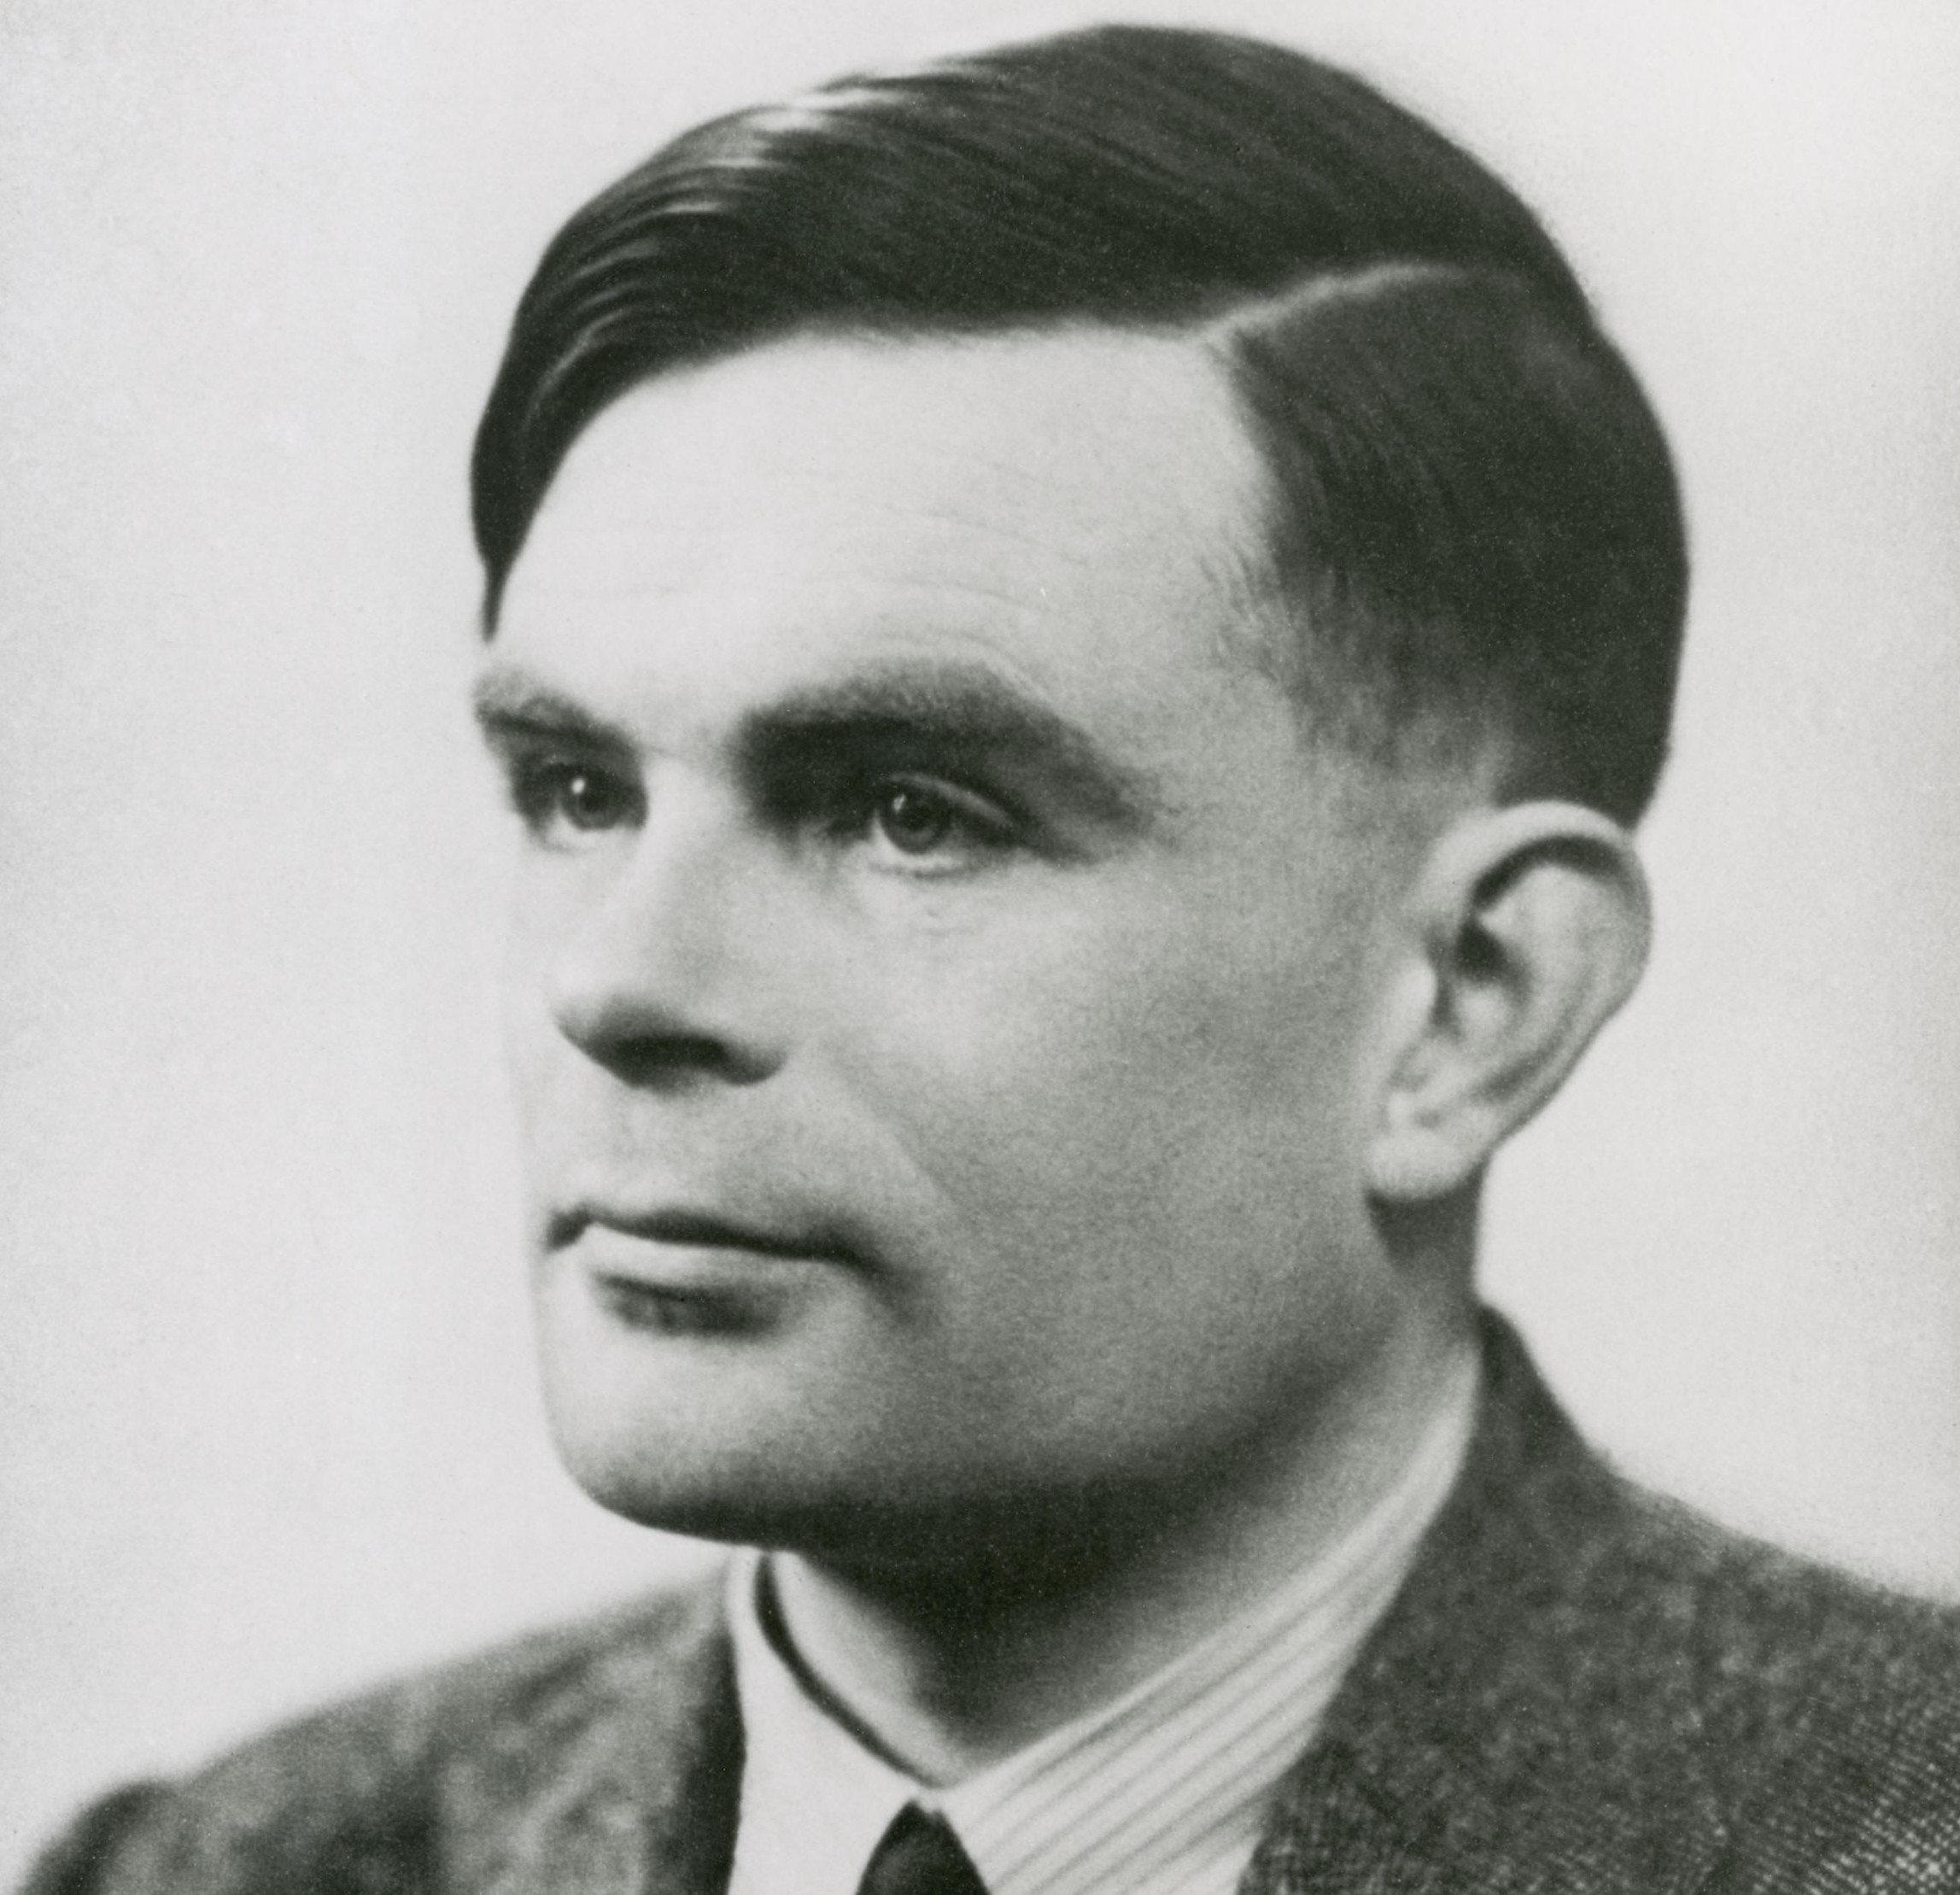
\includegraphics[width=0.77\textwidth]{./images/alan_turing.jpg}
        
        \footnotesize{\textit{`Instead of trying to produce a programme to simulate the adult mind, why not rather try to produce one which simulates the child’s? If this were then subjected to an appropriate course of education one would obtain the adult brain'} Alan Turing, 1950.}
        
    \end{center}
        
    \end{column}
\pause

    \begin{column}{0.48\textwidth}
    \begin{center}
    \textbf{How is it going?}\\
    \vspace{2mm}
        
    
\includegraphics[width=0.95\textwidth]{./images/star_2}
    \end{center}
    \end{column}
\end{columns}

\end{frame}
\begin{frame}
\frametitle{Stroke types}

Most stokes (at least four out of five) are caused by a clot in a blood vessel in the brain. This is also called an \emph{ischaemic} stroke.

\vspace{3mm}



\begin{center}
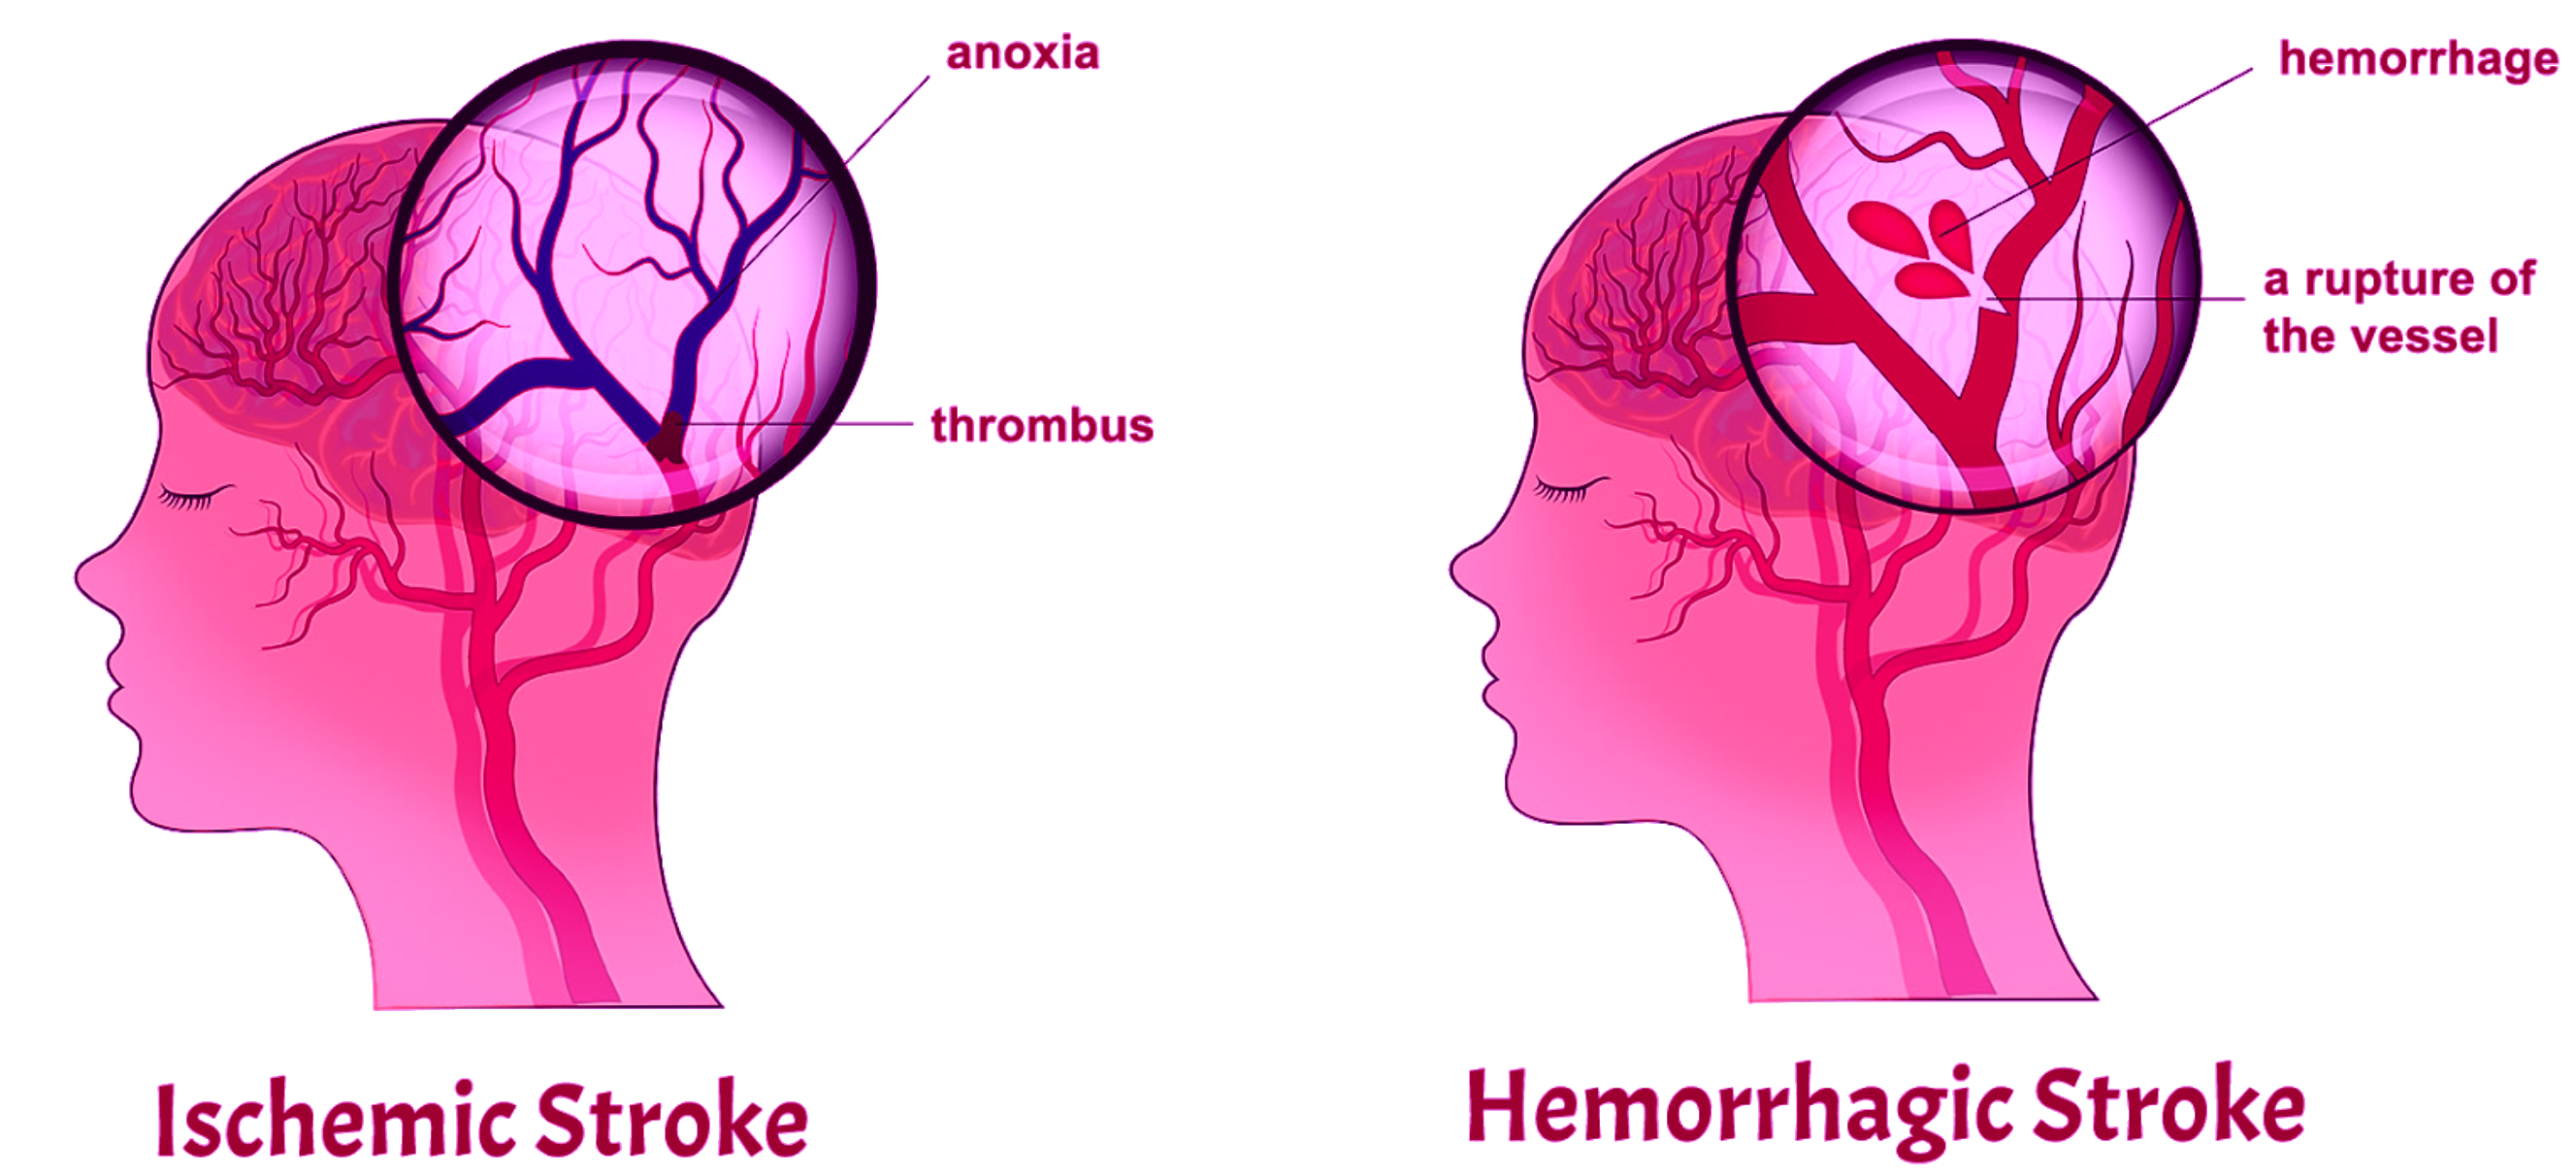
\includegraphics[width=1.0\textwidth]{./images/stroke_types}
\end{center}


\end{frame}

\end{document}